% Compile with XeLaTeX.
\documentclass[UTF8]{ctexart}

\usepackage[a4paper,left=1.15cm,right=1.15cm,top=0.9cm,bottom=0.95cm]{geometry}
\usepackage{graphicx}
\usepackage{hyperref}
\usepackage{enumitem}
\usepackage{tabularx}
\usepackage{array}
\usepackage{xcolor}

\pagenumbering{gobble}
\setlength{\parindent}{0pt}
\setlength{\parskip}{0pt}
\setlength{\tabcolsep}{0pt}
\setlength{\emergencystretch}{2em}
\linespread{1.0}
\urlstyle{same}
\hypersetup{hidelinks}
\setlist[itemize]{leftmargin=1.3em,itemsep=0.14em,topsep=2pt,partopsep=0pt,parsep=0pt}
\definecolor{cvrule}{HTML}{6B7280}
\definecolor{cvmuted}{HTML}{4B5563}

\newcommand{\cvsection}[1]{%
  \vspace{0.35em}
  {\zihao{-3}\bfseries #1\par}
  \vspace{0.1em}
  {\color{cvrule}\hrule height 0.8pt}
  \vspace{0.36em}
}

\newcommand{\cventry}[3]{%
  \begin{tabularx}{\textwidth}{@{}Xr@{}}
    \textbf{#1} & #2 \\
    #3 &
  \end{tabularx}\par
}

\newcommand{\cventryloc}[4]{%
  \begin{tabularx}{\textwidth}{@{}Xr@{}}
    \textbf{#1} & \shortstack[r]{#2\\#3} \\
    #4 &
  \end{tabularx}\par
}

\newcommand{\cventryone}[2]{%
  \begin{tabularx}{\textwidth}{@{}Xr@{}}
    \textbf{#1} & #2
  \end{tabularx}\par
}

\newcommand{\paperentry}[2]{\item #1 \textbf{（#2）}}
\newcommand{\cvmeta}[1]{{\color{cvmuted}\small #1}}
\newcommand{\cvstats}{%
  \vspace{0.45em}
  \begin{center}
  \renewcommand{\arraystretch}{1.05}
  \begin{tabularx}{0.97\textwidth}{>{\centering\arraybackslash}X>{\centering\arraybackslash}X>{\centering\arraybackslash}X>{\centering\arraybackslash}X}
    \textbf{29} & \textbf{920+} & \textbf{2 段} & \textbf{3 个} \\
    {\scriptsize 论文 / 预印本} & {\scriptsize Scholar 引用} & {\scriptsize 研究 / 产业经历} & {\scriptsize 代表性数据项目}
  \end{tabularx}
  \end{center}
  \vspace{-0.15em}
}

% Use a dedicated fallback font for rare Chinese glyphs such as "赟".
\IfFontExistsTF{Noto Serif CJK SC}
  {\newCJKfontfamily\rareglyphfont{Noto Serif CJK SC}[AutoFakeBold=2]}
  {\IfFontExistsTF{Source Han Serif SC}
    {\newCJKfontfamily\rareglyphfont{Source Han Serif SC}[AutoFakeBold=2]}
    {\IfFontExistsTF{Songti SC}
      {\newCJKfontfamily\rareglyphfont{Songti SC}[AutoFakeBold=2]}
      {\IfFontExistsTF{STSong}
        {\newCJKfontfamily\rareglyphfont{STSong}[AutoFakeBold=2]}
        {\IfFontExistsTF{SimSun}
          {\newCJKfontfamily\rareglyphfont{SimSun}[AutoFakeBold=2]}
          {\IfFontExistsTF{Microsoft YaHei}
            {\newCJKfontfamily\rareglyphfont{Microsoft YaHei}[AutoFakeBold=2]}
            {\newCJKfontfamily\rareglyphfont{FandolSong-Regular}[AutoFakeBold=2]}}}}}}

\newcommand{\cvname}{朱{\rareglyphfont 赟}}
\newcommand{\scholarurl}{https://scholar.google.com/citations?user=60HqQsQAAAAJ&hl=zh-CN}

\begin{document}
\fontsize{9.6pt}{11.35pt}\selectfont
\sloppy

\begin{minipage}[c]{0.79\textwidth}
  \centering
  {\zihao{2}\bfseries \cvname\par}
  \vspace{0.35em}
  \cvmeta{电话：15158155897 \,|\, 邮箱：\href{mailto:zhuyun_dcd@zju.edu.cn}{\nolinkurl{zhuyun_dcd@zju.edu.cn}}}\par
  \cvmeta{个人网站：\url{https://zhuyun97.github.io/} \quad Scholar：\href{\scholarurl}{Google Scholar（920+ 引用）}}\par
  {\small 求职方向：多模态数据管线 / 大模型数据工程 / 数据中心化基础设施}
\end{minipage}
\hfill
\begin{minipage}[c]{0.14\textwidth}
  \raggedleft
  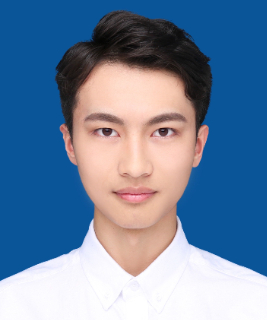
\includegraphics[width=\linewidth]{portrait.png}
\end{minipage}

\cvstats

\cvsection{岗位匹配}
\begin{itemize}
  \item 当前在上海人工智能实验室围绕 VLM post-training 与 multimodal data valuation 开展研究，关注高价值数据识别、数据构建、质量控制与可扩展 data-centric pipelines。
  \item 参与 MMFineReason、OpenDataArena、SciVerse 等项目，覆盖后训练数据价值评估、data genealogy / comparison、多源科学数据标准化与高价值样本构建。
  \item 具备研究与产业两段经历，曾在蚂蚁集团围绕 Foundation Models、Post-training、GraphRAG 推进垂域大模型数据支撑方案；Google Scholar 收录 29 篇论文 / 预印本，引用 920+。
\end{itemize}

\cvsection{工作经历}
\cventryone{上海人工智能实验室（Shanghai AI Lab）}{当前}
\begin{itemize}
  \item 当前任 Junior Researcher，与 Dr. Lijun Wu、Dr. Conghui He 合作开展研究。
  \item 围绕 vision-language models 的 post-training 与 multimodal data valuation 开展研究，关注训练数据价值评估、高价值样本识别与数据构建。
  \item 参与多模态后训练数据流程设计，覆盖数据筛选、质量校验、效果分析与数据迭代，服务真实世界推理与决策任务中的模型对齐需求。
\end{itemize}
\vspace{-0.2em}
\cventryloc{蚂蚁集团}{2024年02月 -- 2025年05月}{杭州}{研究型实习生 \quad 平台事业技术部}
\begin{itemize}
  \item 在 Yongchao Liu 指导下参与支付宝垂域大模型相关工作，围绕 Foundation Models、Post-training 与 GraphRAG 推进研究与实现。
  \item 面向业务需求参与持续预训练、领域微调与数据支撑方案探索，使用 Python 开发研究原型、数据处理脚本与实验流程。
\end{itemize}

\cvsection{项目经历}
\cventryone{MMFineReason}{\href{https://mmfinereason.github.io/}{项目主页}}
\begin{itemize}[leftmargin=1.2em,itemsep=0.1em,topsep=1pt]
  \item 参与大规模多模态推理数据集构建，项目包含 1.8M samples 与 5.1B solution tokens，面向 fine-grained multimodal reasoning 与长链路 CoT supervision。
  \item 参与设计四阶段数据管线：多源数据收集与标准化、高价值样本筛选、CoT rationale 生成、多维质量校验，解决长链路多模态推理数据稀缺与质量不稳问题。
\end{itemize}
\vspace{-0.2em}
\cventryone{OpenDataArena}{\href{https://opendataarena.github.io/}{项目主页}}
\begin{itemize}[leftmargin=1.2em,itemsep=0.1em,topsep=1pt]
  \item 参与构建面向 post-training dataset value 的开放评测与分析项目，包含 leaderboard、data genealogy、data comparison 等核心模块。
  \item 围绕开放数据比较、数据价值评估与训练集工程问题开展工作，为后训练数据选择、数据复用与数据资产化提供支撑。
\end{itemize}
\vspace{-0.2em}
\cventryone{SciVerse}{\href{https://sciverse.opendatalab.com/}{项目主页}}
\begin{itemize}[leftmargin=1.2em,itemsep=0.1em,topsep=1pt]
  \item 参与建设面向 scientific discovery 的 AI-ready multimodal data foundation，覆盖 Scientific Knowledge Base、Scientific Multi-Alignment、Scientific Evolution 等模块。
  \item 围绕 literature、book、patent、code 等多源科学数据开展组织、标准化与对齐，支撑科研场景的数据基础设施与下游应用闭环。
\end{itemize}

\cvsection{技术能力}
\begin{itemize}
  \item Python / Linux / Shell：长期使用 Python 进行研究代码、训练流程与数据处理脚本开发，熟悉 Linux 环境下的实验与数据处理流程，能够编写 Shell 脚本辅助批量任务执行与问题定位。
  \item 数据方向：多模态数据构建、后训练数据选择、数据质量评估、高价值数据识别与生成、GraphRAG、VLM post-training。
  \item 数据系统理解：关注可扩展 data-centric pipelines、benchmark / leaderboard、data genealogy、data comparison、质量校验、版本管理、可追溯与数据复用场景。
\end{itemize}

\cvsection{代表性成果}
{\footnotesize
\begin{itemize}[leftmargin=1.2em,itemsep=0.1em,topsep=1pt]
  \paperentry{GraphCLIP: Enhancing Transferability in Graph Foundation Models for Text-Attributed Graphs}{WWW 2025, 一作}
  \paperentry{Graph Triple Attention Network: A Decoupled Perspective}{KDD 2025, 通讯}
  \paperentry{Meta-Reflection: A Feedback-Free Reflection Learning Framework}{ACL 2025 Main, 二作}
  \paperentry{Bridging Local Details and Global Context in Text-Attributed Graphs}{EMNLP 2024 Main, 共一}
  \paperentry{Efficient Tuning and Inference for Large Language Models on Textual Graphs}{IJCAI 2024, 一作}
  \paperentry{GraphControl: Adding Conditional Control to Universal Graph Pre-trained Models for Graph Domain Transfer Learning}{WWW 2024 Oral, 一作}
\end{itemize}
\textbf{完整论文与预印本列表见：}\href{\scholarurl}{Google Scholar}
}

\cvsection{教育经历}
\cventry{浙江大学}{2020年09月 -- 2025年06月}{计算机科学与技术 博士 计算机科学与技术学院}
\begin{itemize}
  \item DCD Lab 跨媒体组；荣誉\&奖项：省优秀毕业生、陈天洲奖学金、五好研究生、优秀研究生、学术创新能力
\end{itemize}
\vspace{-0.2em}
\cventry{浙江工业大学}{2016年09月 -- 2020年06月}{软件工程 本科 计算机科学与技术学院 / 软件学院}
\begin{itemize}
  \item GPA：4.23/5.0（排名 2/93）；荣誉\&奖项：省优秀毕业生、省政府奖学金、校优秀学生一等奖学金、中国大学生服务外包创新创业大赛国家二等奖
\end{itemize}

\cvsection{专业竞赛}
\cventryone{DCVLR @ NeurIPS 2025——Data Curation for Vision Language Reasoning}{2025年06月 -- 2025年11月}
\begin{itemize}
  \item Final Leaderboard 第四名（Team: ZhuYun - PJLab），准确率 38.84\%，较 baseline 提升 0.01\%。
  \item 面向 vision-language reasoning 任务进行数据构建与策划，围绕可复现的数据选择与生成策略提交数据集与技术报告。
\end{itemize}
\vspace{-0.2em}
\cventryone{KDD CUP 2024——利用大语言模型辅助在线购物}{2024年05月 -- 2024年07月}
\begin{itemize}
  \item 五个赛道平均排名第三（3/508），多语言赛道获得 ``Best Student Awards''。
  \item 相关工作产出 KDD 2024 Workshop（Oral）论文。
\end{itemize}
\vspace{-0.2em}
\cventryone{AgentSociety Challenge @ WWW 2025——利用Agent进行商品推荐}{2025年01月 -- 2025年02月}
\begin{itemize}
  \item 排名第五（5/76）。
\end{itemize}
\vspace{-0.2em}
\cventryone{中国大学生服务外包创新创业大赛——网络零售平台商品分类}{2019年03月 -- 2019年05月}
\begin{itemize}
  \item 解决电子商品短文本千分类难题，获国家二等奖。
\end{itemize}

\end{document}
